\documentclass[12pt,a4paper,openright,twoside]{book}
\usepackage[utf8]{inputenc}
\usepackage{phd-thesis}
\usepackage{code-lstlistings}
\usepackage{notes}
\usepackage{shortcuts}

\school{\unibo}
\programme{Dottorato di Ricerca in Data Science and Computation}
\title{Fancy Title Here}
\author{Candidate Name Here}
\date{\today}
\contestsector{09/H1 -- Sistemi di Elaborazione delle Informazioni}
\scientificsector{ING-INF/05 -- Sistemi di Elaborazione delle Informazioni}
\coordinator{Andrea Cavalli}
\supervisor{Supervisor Here}
\cycle{XXXIII}
\examyear{2022}

\mainlinespacing{1.241} % line spacing in mainmatter, comment to default (1)

\begin{document}
	
\frontmatter\frontispiece

\begin{abstract}	
Max 2000 characters, strict.
\end{abstract}

\begin{dedication} % this is optional
Optional. Max a few lines.
\end{dedication}

\begin{acknowledgements} % this is optional
Optional. Max 1 page.
\end{acknowledgements}

%----------------------------------------------------------------------------------------
\tableofcontents   
\listoffigures     % (optional) comment if empty
\lstlistoflistings % (optional) comment if empty
%----------------------------------------------------------------------------------------

\mainmatter

%----------------------------------------------------------------------------------------
\chapter{Introduction}
\label{chap:introduction}
%----------------------------------------------------------------------------------------

Write your intro here.
\sidenote{Add sidenotes in this way. They are named after the author of the thesis}

\paragraph{Structure of the Thesis}

\note{Racall to describe the structure of the paper}

\part{First Part}

\chapter{State of the art}

I suggest referencing stuff as follows: \cref{fig:random-image} or \Cref{fig:random-image}

\begin{figure}
    \centering
    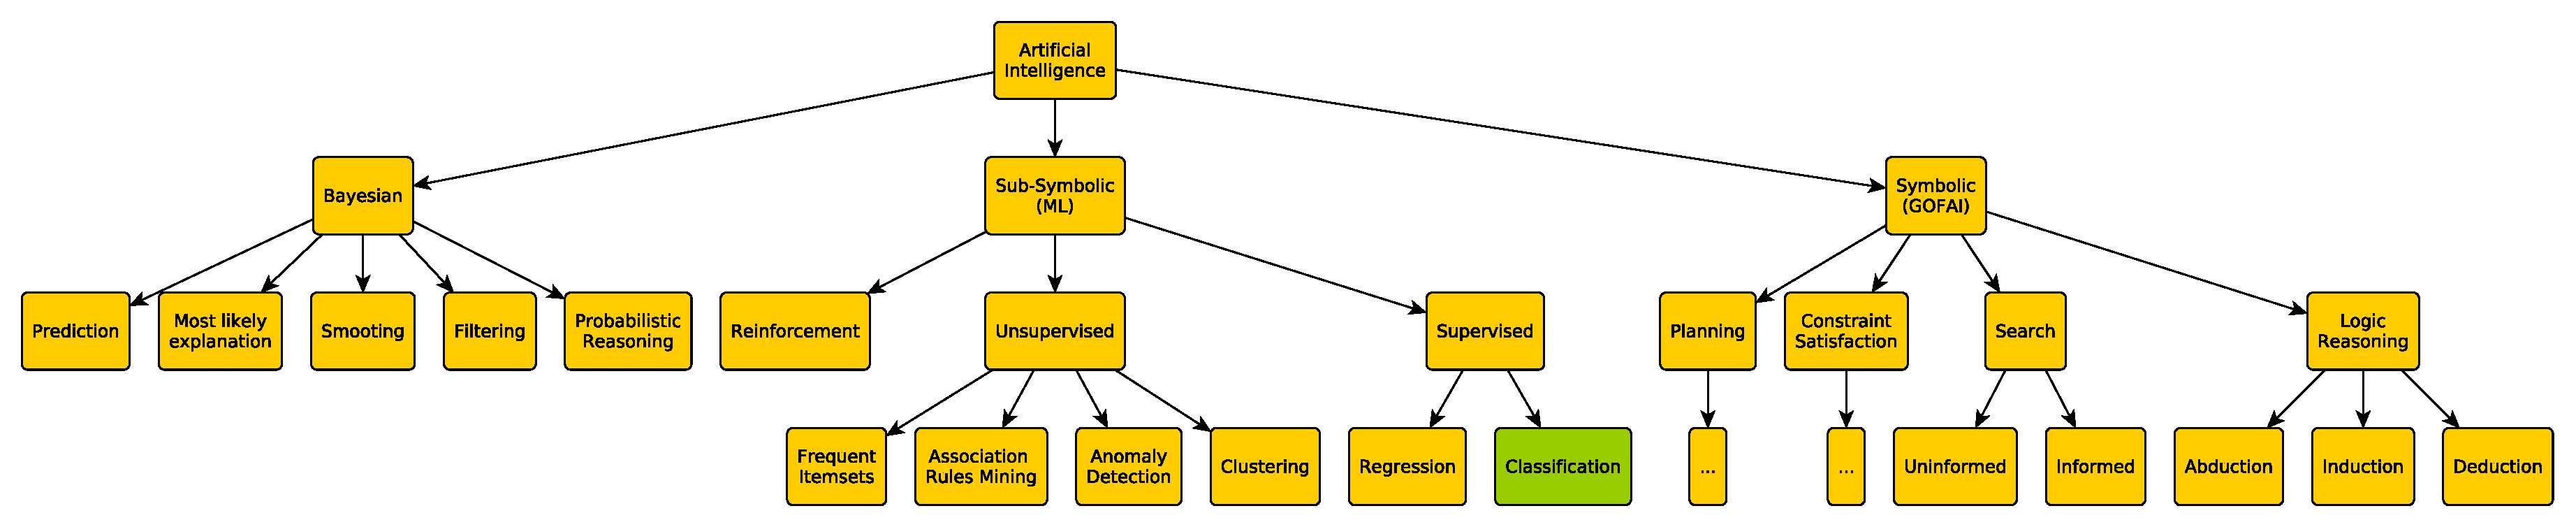
\includegraphics[width=.8\linewidth]{figures/random-image.pdf}
    \caption{Some random image}
    \label{fig:random-image}
\end{figure}

References to URLs are better stored in footnotes\footnote{
\url{https://danysk.github.io/2020/05/08/bibliography/}
},
leaving the bibliography only for papers such as \cite{LevesqueB87}.

\section{Some cool topic}

\part{Second Part}

\chapter{Contribution}

You may also put some code snippet (which is NOT float by default), eg: \cref{lst:random-code}.

\lstinputlisting[float,language=Java,label={lst:random-code}]{listings/HelloWorld.java}

\section{Fancy formulas here}

%----------------------------------------------------------------------------------------
% BIBLIOGRAPHY
%----------------------------------------------------------------------------------------

\backmatter

\part*{}

\bibliographystyle{alpha}
\bibliography{phd-thesis}

\end{document}
